\documentclass[12pt]{exam}
\usepackage{amssymb}
\usepackage{amsmath}
\usepackage{graphicx}
\usepackage{hyperref}
\usepackage{soul}
\newcommand{\ppp}{\par \noindent}
\newcommand{\R}{\mathbb{R}}
\newcommand{\ds}{\displaystyle}
\newcommand{\PS}{\mathcal{P}}
\pagestyle{empty} 

\begin{document}

\centerline{\textbf{CSE 373 HW5 Writeup}}
\centerline{By Stephen Hung}

\begin{questions}


\question {\bf Topological Sort}

Queue is bottom on the left and top on the right

% Question 1 on CSE 373 Homework 5 Writeup
\begin{tabular}{ |c|c|c|c|c|c|c|c| }
\hline
vertex & A & B & C & D & E & F & G \\
\hline
in-degree & 0 & 1 & 1 & 2 & 2 & 1 & 0 \\
\hline
\end{tabular}
$\rightarrow$ 
Queue: 
\begin{tabular}{ c c c c c c c c }
\hline
G & A \\
\hline
\end{tabular}
$\rightarrow$ Output "A" $\rightarrow$

\begin{tabular}{ |c|c|c|c|c|c|c|c| }
\hline
vertex & B & C & D & E & F & G \\
\hline
in-degree & 0 & 1 & 1 & 2 & 1 & 0 \\
\hline
\end{tabular}
$\rightarrow$ 
Queue: 
\begin{tabular}{ c c c c c c c c }
\hline
B & G \\
\hline
\end{tabular}
$\rightarrow$ Output "G" $\rightarrow$

\begin{tabular}{ |c|c|c|c|c|c|c|c| }
\hline
vertex & B & C & D & E & F \\
\hline
in-degree & 0 & 1 & 1 & 2 & 0 \\
\hline
\end{tabular}
$\rightarrow$ 
Queue: 
\begin{tabular}{ c c c c c c c c }
\hline
F & B \\
\hline
\end{tabular}
$\rightarrow$ Output "B" $\rightarrow$

\begin{tabular}{ |c|c|c|c|c|c|c|c| }
\hline
vertex & C & D & E & F \\
\hline
in-degree & 1 & 0 & 1 & 0 \\
\hline
\end{tabular}
$\rightarrow$ 
Queue: 
\begin{tabular}{ c c c c c c c c }
\hline
D & F \\
\hline
\end{tabular}
$\rightarrow$ Output "F" $\rightarrow$

\begin{tabular}{ |c|c|c|c|c|c|c|c| }
\hline
vertex & C & D & E  \\
\hline
in-degree & 1 & 0 & 1  \\
\hline
\end{tabular}
$\rightarrow$ 
Queue: 
\begin{tabular}{ c c c c c c c c }
\hline
D \\
\hline
\end{tabular}
$\rightarrow$ Output "D" $\rightarrow$

\begin{tabular}{ |c|c|c|c|c|c|c|c| }
\hline
vertex & C & E \\
\hline
in-degree & 1 & 0 \\
\hline
\end{tabular}
$\rightarrow$ 
Queue: 
\begin{tabular}{ c c c c c c c c }
\hline
E \\
\hline
\end{tabular}
$\rightarrow$ Output "E" $\rightarrow$

\begin{tabular}{ |c|c|c|c|c|c|c|c| }
\hline
vertex & C  \\
\hline
in-degree & 0  \\
\hline
\end{tabular}
$\rightarrow$ 
Queue: 
\begin{tabular}{ c c c c c c c c }
\hline
C \\
\hline
\end{tabular}
$\rightarrow$ Output "C" $\rightarrow$

{\bf Output: A, G, B, F, D, E, C}

\question 
{\bf Minimum Spanning Trees}
\begin{parts}

\part Kruskal's Algorithm

\begin{tabular}{|c|c|c|c|}
\hline
Cost & Edges & & \\
\hline
1: & (B,E) & (C,G) & (D,G) \\
2: & (A,B) & (C,D) & (E,F) \\ 
3: & (A,E) & (B,F) & (E,G) \\ 
4: & (A,D) & (F,G) & \\
\hline
\end{tabular}
$\rightarrow$ Output $\#1$ edge (B,E)

\begin{tabular}{|c|c|c|c|}
\hline
Cost & Edges & & \\
\hline
1: & \st{(B,E)} & (C,G) & (D,G) \\
2: & (A,B) & (C,D) & (E,F) \\ 
3: & (A,E) & (B,F) & (E,G) \\ 
4: & (A,D) & (F,G) & \\
\hline
\end{tabular}
$\rightarrow$ Output $\#2$ edge (C,G)

\begin{tabular}{|c|c|c|c|}
\hline
Cost & Edges & & \\
\hline
1: & \st{(B,E)} & \st{(C,G)} & (D,G) \\
2: & (A,B) & (C,D) & (E,F) \\ 
3: & (A,E) & (B,F) & (E,G) \\ 
4: & (A,D) & (F,G) & \\
\hline
\end{tabular}
$\rightarrow$ Output $\#3$ edge (D,G)

\begin{tabular}{|c|c|c|c|}
\hline
Cost & Edges & & \\
\hline
1: & \st{(B,E)} & \st{(C,G)} & \st{(D,G)} \\
2: & (A,B) & (C,D) & (E,F) \\ 
3: & (A,E) & (B,F) & (E,G) \\ 
4: & (A,D) & (F,G) & \\
\hline
\end{tabular}
$\rightarrow$ Output $\#4$ edge (A,B)

\begin{tabular}{|c|c|c|c|}
\hline
Cost & Edges & & \\
\hline
1: & \st{(B,E)} & \st{(C,G)} & \st{(D,G)} \\
2: & \st{(A,B)} & (C,D) & (E,F) \\ 
3: & (A,E) & (B,F) & (E,G) \\ 
4: & (A,D) & (F,G) & \\
\hline
\end{tabular}
$\rightarrow$ Output $\#5$ edge (E,F) 

Edge (C,D) is not outputted because it contains the vertices C and D which have already been processed before.

\begin{tabular}{|c|c|c|c|}
\hline
Cost & Edges & & \\
\hline
1: & \st{(B,E)} & \st{(C,G)} & \st{(D,G)} \\
2: & \st{(A,B)} & \st{(C,D)} & \st{(E,F)} \\ 
3: & (A,E) & (B,F) & (E,G) \\ 
4: & (A,D) & (F,G) & \\
\hline
\end{tabular}
$\rightarrow$ Output $\#6$ edge (E,G)

Edge (A,E) and (B,F) are not outputted because the vertices A,B,E, and F have already been
processed before.

\begin{tabular}{|c|c|c|c|}
\hline
Cost & Edges & & \\
\hline
1: & \st{(B,E)} & \st{(C,G)} & \st{(D,G)} \\
2: & \st{(A,B)} & \st{(C,D)} & \st{(E,F)} \\ 
3: & \st{(A,E)} & \st{(B,F)} & \st{(E,G)} \\ 
4: & (A,D) & (F,G) & \\
\hline
\end{tabular}

The amount of edges $= |V| -1 = 6$ so Kruskal's algorithm stops.

{\bf Edge Number and Output: $\#1:$(B,E), $\#2:$(C,G), $\#3:$(D,G), $\#4:$(A,B), $\#5:$(E,F), $\#6:$(E,G) }

Minimum Spanning Tree:

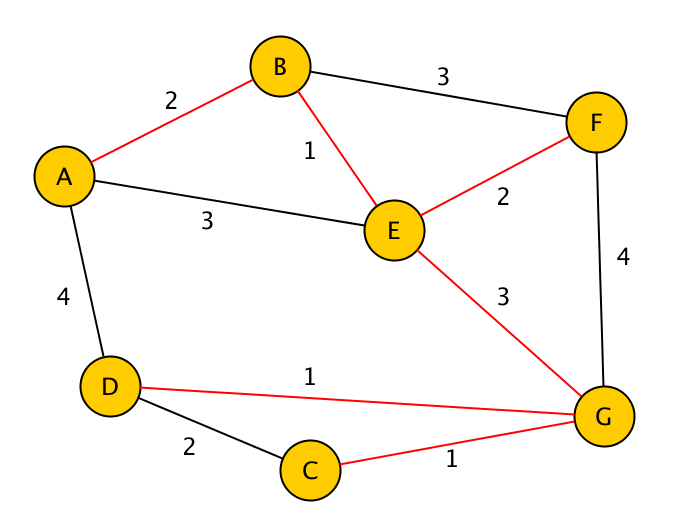
\includegraphics[scale=0.5]{hw5writeup2a.png}

\part Prim's Algorithm

\begin{tabular}{|c c c c|}
\hline
Vertex & Known & Cost & Path \\
A & Y & 0 & \\
B & & 2 & A \\
C & & $\infty$ & \\
D & & 4 & A \\
E & & 3 & A \\
F & & $\infty$ & \\
G & & $\infty$ & \\
\hline
\end{tabular}
$\rightarrow$ Output Edge $\#1:$(A,B) 

\begin{tabular}{|c c c c|}
\hline
Vertex & Known & Cost & Path \\
A & Y & 0 & \\
B & Y & 2 & A \\
C & & $\infty$ & \\
D & & 4 & A \\
E & & 1 & B \\
F & & 3 & B \\
G & & $\infty$ & \\
\hline
\end{tabular}
$\rightarrow$ Output Edge $\#2:$(B,E) 

\begin{tabular}{|c c c c|}
\hline
Vertex & Known & Cost & Path \\
A & Y & 0 & \\
B & Y & 2 & A \\
C & & $\infty$ & \\
D & & 4 & A \\
E & Y & 1 & B \\
F & & 2 & E \\
G & & 3 & E \\
\hline
\end{tabular}
$\rightarrow$ Output Edge $\#3:$(E,F) 

\begin{tabular}{|c c c c|}
\hline
Vertex & Known & Cost & Path \\
A & Y & 0 & \\
B & Y & 2 & A \\
C & & $\infty$ & \\
D & & 4 & A \\
E & Y & 1 & B \\
F & Y & 2 & E \\
G & & 3 & E \\
\hline
\end{tabular}
$\rightarrow$ Output Edge $\#4:$(E,G) 

\begin{tabular}{|c c c c|}
\hline
Vertex & Known & Cost & Path \\
A & Y & 0 & \\
B & Y & 2 & A \\
C & & 1 & G \\
D & & 1 & G \\
E & Y & 1 & B \\
F & Y & 2 & E \\
G & Y & 3 & E \\
\hline
\end{tabular}
$\rightarrow$ Output Edge $\#5:$(G,C) 

\begin{tabular}{|c c c c|}
\hline
Vertex & Known & Cost & Path \\
A & Y & 0 & \\
B & Y & 2 & A \\
C & Y & 1 & G \\
D & & 1 & G \\
E & Y & 1 & B \\
F & Y & 2 & E \\
G & Y & 3 & E \\
\hline
\end{tabular}
$\rightarrow$ Output Edge $\#6:$(G,D) 

\begin{tabular}{|c c c c|}
\hline
Vertex & Known & Cost & Path \\
A & Y & 0 & \\
B & Y & 2 & A \\
C & Y & 1 & G \\
D & Y & 1 & G \\
E & Y & 1 & B \\
F & Y & 2 & E \\
G & Y & 3 & E \\
\hline
\end{tabular}

Because all of the nodes have been processed, the algorithm stops.

{\bf Edge Number and Output: $\#1:$(A,B), $\#2:$(B,E), $\#3:$(E,F), $\#4:$(E,G), $\#5:$(G,C), $\#6:$(G,D) }

Minimum Spanning Tree:

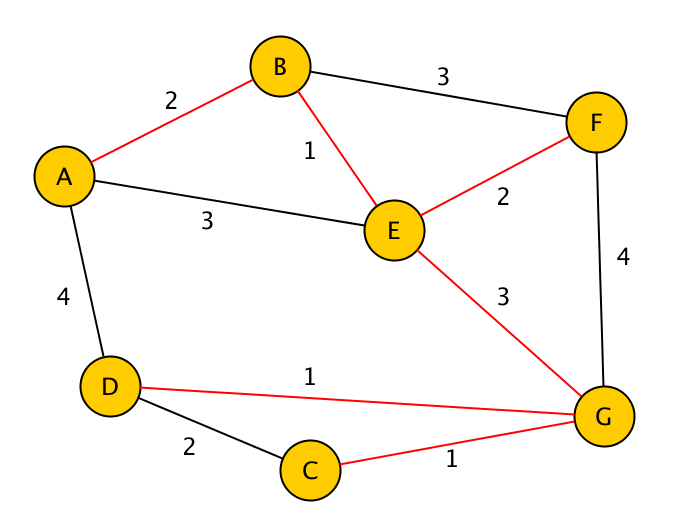
\includegraphics[scale=0.5]{hw5writeup2a.png}

\end{parts}

\question {\bf Dijkstra’s and Negative Edges:}

\begin{parts}

\part No. Dijkstra's Algorithm only cares about the weight of the edges instead of the number of the edges. For example in the following graph the shortest path from A to E will give A - B - C - D - E 

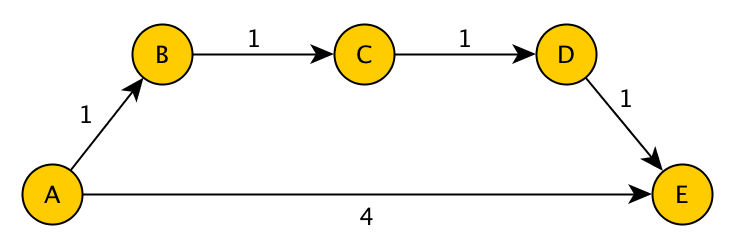
\includegraphics[scale=0.5]{hw5writeup3a.png}

However, the path A - E has the same weight but fewer edges yet it is not chosen. A way to modify Dijkstra's Algorithm is to keep track of both the total cost from the source and the number of edges from the source. Therefore when deciding which node to process next, find the minimum cost and the minimum number of edges from the source. 

\part The following is a graph with a negative cost edge where Dijkstra's Algorithm gives the wrong answer for the path from A to B.

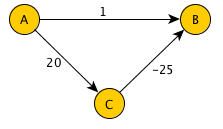
\includegraphics[scale=0.5]{hw5writeup3b.png}

Dijkstra's Algorithm fails this example because when starting from A, Dijkstra's Algorithm chooses the adjacent edge with the lowest cost. This is A to B with a cost of 1 since A to C has a cost of 20. Once it has done so, the vertex B is marked known like so:

\begin{tabular}{| c c c c |}
\hline
Vertex & Known & Cost & Path \\
A & Y & 0 & \\
B & Y & 1 & A \\
C & & 20 & A \\
\hline
\end{tabular}

Afterwards, Dijkstra's Algorithm processes vertex C and quits, since there are no more unknown vertices.

\begin{tabular}{| c c c c |}
\hline
Vertex & Known & Cost & Path \\
A & Y & 0 & \\
B & Y & 1 & A \\
C & Y & 20 & A \\
\hline
\end{tabular}

This results in the path A to B with a cost of 1, but the path A to C to B has a cost of $-5$ which is actually the lowest cost path. The reason why when processing C, the vertex B's cost and path are not updated is because B is already marked known and thus Dijkstra fails.

\part For this problem I use the same graph from part 3b since it has negative-cost edges but has no negative-cost cycles. I then add 30 to all the edges in order to make sure the edge costs are positive.

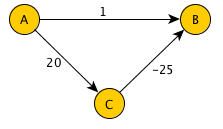
\includegraphics[scale=0.5]{hw5writeup3b.png}$\rightarrow$
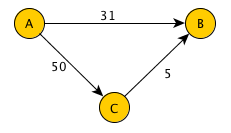
\includegraphics[scale=0.5]{hw5writeup3c.png}

After running Dijkstra's Algorithm and subtracting 30 cost from each the cost and path for each vertex is as follows: 

\begin{tabular}{| c c c c |}
\hline
Vertex & Known & Cost & Path \\
A & Y & 30 & \\
B & Y & 31 & A \\
C & Y & 50 & A \\
\hline
\end{tabular}
$\rightarrow$
\begin{tabular}{| c c c c |}
\hline
Vertex & Known & Cost & Path \\
A & Y & 0 & \\
B & Y & 1 & A \\
C & Y & 20 & A \\
\hline
\end{tabular}

Thus Dijkstra's Algorithm would still return the path A to B. As shown in the previous part (3b), the actual correct path is A to C to B, but Dijkstra's Algorithm still returns A to B. This is because, B is "known" first and thus when C is processed, the negative edge from C to B is ignored thus ignoring the A to C to B path.

A general explanation for why this technique does not work is that the negative weight of an edge was why it would be a part of the original least cost path. This is due to the fact that no matter the weight of the edge before, the negative weight of the edge can reduce the total cost till it is the smallest. Therefore, when all edges become positive, the ability of the negative weight dissapears and thus the path is no longer the least cost path.

\end{parts}

\question {\bf Testing:}

Most of my testing was done using the provided edge.txt and vertex.txt. First I manually computed several paths of varying lengths. An example of this is the path from ORD to SEA which should be a path containing five vertices including the source and destination and has a cost of 541. Afterwards, I ran Dijkstra's Algorithm in order to determine that the paths I manually computed and the paths that were returned were the same. 

I also tested for boundary cases such as when a vertex is not connected to any other vertices. So for example, I added SJC to the vertex.txt and tried to find the shortest path from SEA to SJC which should return an error. Another case I tested for was the IllegalArgumentException thrown when a vertex doesn't exist.

I also tested for cyclic graphs and when the source and destination vertex are the same. 


\end{questions}
\end{document}
